\documentclass[letterpaper]{report}
\usepackage[letterpaper]{geometry}
\usepackage{vhistory}
\usepackage{graphicx}
\graphicspath{ {./images/} }
%\usepackage{epstopdf }
\usepackage{indentfirst}
%\usepackage{amsmath}
%\usepackage{gensymb}
\usepackage{multirow}
%\usepackage{pdfpages}
\usepackage{float}


\setcounter{tocdepth}{3}
\setcounter{secnumdepth}{3}

\begin{document}

\pagenumbering{roman}
	\title{ViSOR by Krueger Labs}
	\author{in collaboration with \\ Sevun Scientific, Inc.}
	\date{\today \\ Version 0.0.1}
\maketitle

%\thispagestyle{empty}

\newpage
% Start of the revision history table
\begin{versionhistory}
  \vhEntry{0.0.1}{2018-04-18}{BD}{Hello World}
\end{versionhistory}
%\setcounter{table}{0} % added because version history shows up as a table

\newpage
\tableofcontents

\newpage
\listoffigures

\newpage
\listoftables

\newpage
\pagenumbering{arabic}
\setcounter{page}{1}

\chapter{Processor}
Lorem ipsum dolor sit amet, consectetur adipiscing elit. Pellentesque nisl mi, sagittis a placerat eget, vulputate id ante. Maecenas non sapien turpis. Morbi faucibus a magna et lobortis. Morbi porttitor eget est at sollicitudin. Etiam arcu justo, tempus et sagittis in, eleifend vel mi. Nunc vestibulum eget magna vel lobortis. Fusce tincidunt congue mi sagittis ornare. Duis a velit et turpis condimentum blandit quis at orci.

%*********************************************************
\chapter{Sensors}
The BRKT-STBC-AGM01 contains a FXOS8700C and FXAS21002C sensors in a breakout board package.  Hookup Notes by Pin:

[1] Bleh

[2] Blah


\begin{figure}[H]
	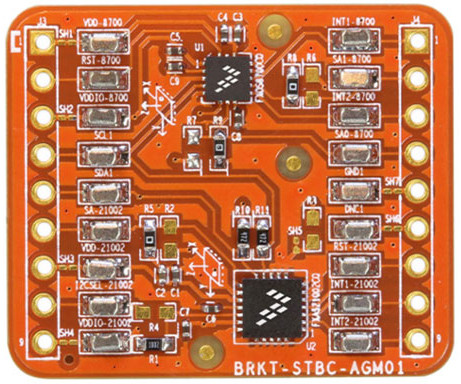
\includegraphics[scale=0.25]{brkt-stbc-agm01}
	\centering
	\caption{BRKT-STBC-AGM01 Board}
\end{figure}

\begin{table}[H]
	\centering
	\begin{tabular}{ | l | l | l |} \hline
	Pin	& J3			&J4			\\ \hline \hline
	1	& VDD\_8700	& INT1\_8700	\\ \hline
	2	& RST\_8700		& SA1\_8700		\\ \hline
	3	& VDDIO\_8700	& INT2\_8700	\\ \hline
	4	& SCL1		& SA0\_8700		\\ \hline
	5	& SDA1		& GND			\\ \hline
	6	& SA\_21002		& DNC			\\ \hline
	7	& VDD\_21002	& RST\_21002	\\ \hline
	8	& SPI\_CSB\_21002	& INT1\_21002	\\ \hline
	9	& VDDIO\_21002	& INT2\_21002	\\ \hline
    \end{tabular}
    \caption{BRKT-STBC-AGM01 Pinout}
\end{table}



\section{Gyroscope}
FXAS21002C is a small, low-power, yaw, pitch, and roll angular rate gyroscope with 16 bit ADC resolution. The full-scale range is adjustable from ±250°/s to ±2000°/s. It features both I2C and SPI interfaces.

FXAS21002C is capable of measuring angular rates up to ±2000°/s, with output data rates (ODR) from 12.5 to 800 Hz. An integrated Low-Pass Filter (LPF) allows the host application to
limit the digital signal bandwidth. The device may be configured to generate an interrupt when a user-programmable angular rate threshold is crossed on any one of the enabled axes.

FXAS21002C is available in a plastic, 24-lead QFN package; the device is guaranteed to operate over the extended temperature range of –40 °C to +85 °C.

\section{Accelerometer and Magnetometer}
Lorem ipsum dolor sit amet, consectetur adipiscing elit. Pellentesque nisl mi, sagittis a placerat eget, vulputate id ante. Maecenas non sapien turpis. Morbi faucibus a magna et lobortis. Morbi porttitor eget est at sollicitudin. Etiam arcu justo, tempus et sagittis in, eleifend vel mi. Nunc vestibulum eget magna vel lobortis. Fusce tincidunt congue mi sagittis ornare. Duis a velit et turpis condimentum blandit quis at orci.

%*********************************************************
\chapter{Cameras}
Lorem ipsum dolor sit amet, consectetur adipiscing elit. Pellentesque nisl mi, sagittis a placerat eget, vulputate id ante. Maecenas non sapien turpis. Morbi faucibus a magna et lobortis. Morbi porttitor eget est at sollicitudin. Etiam arcu justo, tempus et sagittis in, eleifend vel mi. Nunc vestibulum eget magna vel lobortis. Fusce tincidunt congue mi sagittis ornare. Duis a velit et turpis condimentum blandit quis at orci.

%*********************************************************
\chapter{Power}
Lorem ipsum dolor sit amet, consectetur adipiscing elit. Pellentesque nisl mi, sagittis a placerat eget, vulputate id ante. Maecenas non sapien turpis. Morbi faucibus a magna et lobortis. Morbi porttitor eget est at sollicitudin. Etiam arcu justo, tempus et sagittis in, eleifend vel mi. Nunc vestibulum eget magna vel lobortis. Fusce tincidunt congue mi sagittis ornare. Duis a velit et turpis condimentum blandit quis at orci.

\end{document}